\chapter{Átomos e moléculas}\label{ch:g7:atoms-and-molecules}

Pegue uma gota de água e corte-a em duas. Cada metade continua sendo
água. Corte uma metade em duas de novo, e de novo, e de novo. Daria para
continuar para sempre, ou você chegaria a um pedaço tão pequeno que
cortá-lo mais uma vez daria uma coisa que já não é água? Por volta de
400~a.C., o pensador grego Demócrito arriscou a resposta: a matéria é
feita de pedacinhos minúsculos que não podem ser cortados, que ele
chamou de \emph{\omterm{def:g7:atoms-and-molecules:atom}{átomos}}, do grego ``indivisível''. Foram precisos mais de
dois mil anos, e o trabalho dos químicos do século XIX, para transformar
esse palpite em ciência. Este capítulo descreve esses pedacinhos --- os
\omterm{def:g7:atoms-and-molecules:atom}{átomos} --- e o modo como eles se agrupam em \omterm{def:g7:atoms-and-molecules:molecule}{moléculas}.

\begin{recall}
Uma \omterm{def:g6:pure-substances-and-mixtures:pure-substance}{substância pura}, como a água ou o oxigênio, é formada por uma única
\omterm{def:g6:pure-substances-and-mixtures:species}{espécie química}; uma \omterm{def:g6:pure-substances-and-mixtures:mixture}{mistura}, como o \omterm{def:g4:air-a-mixture-of-gases:air}{ar}, contém várias
(\cref{ch:g6:pure-substances-and-mixtures}). O \omterm{def:g4:air-a-mixture-of-gases:air}{ar} tem cerca de quatro
quintos de nitrogênio e um quinto de oxigênio
(\cref{ch:g4:air-a-mixture-of-gases}).
\end{recall}

\section{Os átomos}

\begin{definition}[Átomo]\label{def:g7:atoms-and-molecules:atom}
Toda a matéria é construída a partir de partículas extremamente
pequenas chamadas \emph{átomos}\index{atomo@átomo}. Na natureza existem só
cerca de cem tipos diferentes de átomos, e toda substância --- a água, o
\omterm{def:g4:air-a-mixture-of-gases:air}{ar}, o ferro, o açúcar, o nosso próprio corpo --- é feita de átomos de
alguns desses tipos.
\end{definition}

\begin{proposition}[Os átomos são minúsculos]\label{prop:g7:atoms-and-molecules:tiny}
% ledger: const:a0, earth:diameter (8 cm apple: 12756 km / 8 cm = 1.6 x 10^8;
% 0.1-0.15 nm x 1.6 x 10^8 = 1.7-2.4 cm, a small cherry)
O menor \omterm{def:g7:atoms-and-molecules:atom}{átomo}, o \omterm{def:g7:atoms-and-molecules:atom}{átomo} de hidrogênio, mede cerca de um décimo de
milionésimo de milímetro de diâmetro; os outros são no máximo algumas
vezes maiores. Dez milhões de \omterm{def:g7:atoms-and-molecules:atom}{átomos} de hidrogênio enfileirados
formariam uma linha de um milímetro. Para imaginar: se uma maçã fosse
aumentada até o tamanho da Terra, cada um dos seus \omterm{def:g7:atoms-and-molecules:atom}{átomos} teria mais ou
menos o tamanho de uma cereja pequena.
\end{proposition}

\begin{remark}[Vistos sem ser vistos]\label{rem:g7:atoms-and-molecules:seen}
Nenhum microscópio que usa luz consegue mostrar um \omterm{def:g7:atoms-and-molecules:atom}{átomo}: os \omterm{def:g7:atoms-and-molecules:atom}{átomos} são
muito menores do que as ondas da luz. Desde a década de 1980,
microscópios especiais que tateiam uma superfície com uma ponta
extremamente fina produzem imagens em que \omterm{def:g7:atoms-and-molecules:atom}{átomos} isolados aparecem como
pequenas saliências.
\end{remark}

\begin{definition}[Símbolo de um átomo]\label{def:g7:atoms-and-molecules:symbol}
Cada tipo de \omterm{def:g7:atoms-and-molecules:atom}{átomo} tem um nome e um
\emph{símbolo}\index{simbolo de um atomo@símbolo de um átomo}: uma letra maiúscula, às vezes
seguida de uma letra minúscula. O símbolo é o mesmo em todas as
línguas.
\end{definition}

\begin{center}
\small
\begin{tabular}{llll|llll}
\hline
\omterm{def:g7:atoms-and-molecules:atom}{átomo} & \omterm{def:g7:atoms-and-molecules:symbol}{símbolo} & & cor no modelo & \omterm{def:g7:atoms-and-molecules:atom}{átomo} & \omterm{def:g7:atoms-and-molecules:symbol}{símbolo} & & cor no modelo \\
\hline
hidrogênio & \ce{H} & \tikz\node[aH]{}; & branco & sódio & \ce{Na} & \tikz\node[aNa]{}; & roxo \\
carbono & \ce{C} & \tikz\node[aC]{}; & preto & enxofre & \ce{S} & \tikz\node[aS]{}; & amarelo \\
nitrogênio & \ce{N} & \tikz\node[aN]{}; & azul & cloro & \ce{Cl} & \tikz\node[aCl]{}; & verde \\
oxigênio & \ce{O} & \tikz\node[aO]{}; & vermelho & ferro, cobre & \ce{Fe}, \ce{Cu} & & --- \\
\hline
\end{tabular}
\end{center}

\begin{remark}[De onde vêm os símbolos]\label{rem:g7:atoms-and-molecules:latin}
A maioria dos \omterm{def:g7:atoms-and-molecules:symbol}{símbolos} são as primeiras letras do nome: \ce{H} para o
hidrogênio, \ce{C} para o carbono, \ce{O} para o oxigênio. Alguns vêm de
um nome mais antigo, em latim: \ce{Na} para o sódio (\emph{natrium}),
\ce{Fe} para o ferro (\emph{ferrum}), \ce{Cu} para o cobre
(\emph{cuprum}). A segunda letra é sempre minúscula: \ce{Co} é o \omterm{def:g7:atoms-and-molecules:atom}{átomo}
de cobalto, enquanto CO, com O maiúsculo, é uma coisa totalmente
diferente.
\end{remark}

\begin{history}[Os átomos de Dalton, 1808]
Em 1808, o químico John Dalton publicou uma tabela dos \omterm{def:g7:atoms-and-molecules:atom}{átomos} então
conhecidos, cada um desenhado como um pequeno círculo com um sinal
próprio. Ele foi o primeiro a dizer que todos os \omterm{def:g7:atoms-and-molecules:atom}{átomos} de um mesmo tipo
têm o mesmo peso, e que os químicos podiam comparar esses pesos. Mas ele
também supôs que a água era um \omterm{def:g7:atoms-and-molecules:atom}{átomo} de hidrogênio ligado a um \omterm{def:g7:atoms-and-molecules:atom}{átomo} de
oxigênio; foram precisos mais cinquenta anos para os químicos
concordarem que uma \omterm{def:g7:atoms-and-molecules:molecule}{molécula} de água contém \emph{dois} \omterm{def:g7:atoms-and-molecules:atom}{átomos} de
hidrogênio.
\end{history}

\begin{omfigure}
\begin{minipage}[b]{0.3\linewidth}\centering
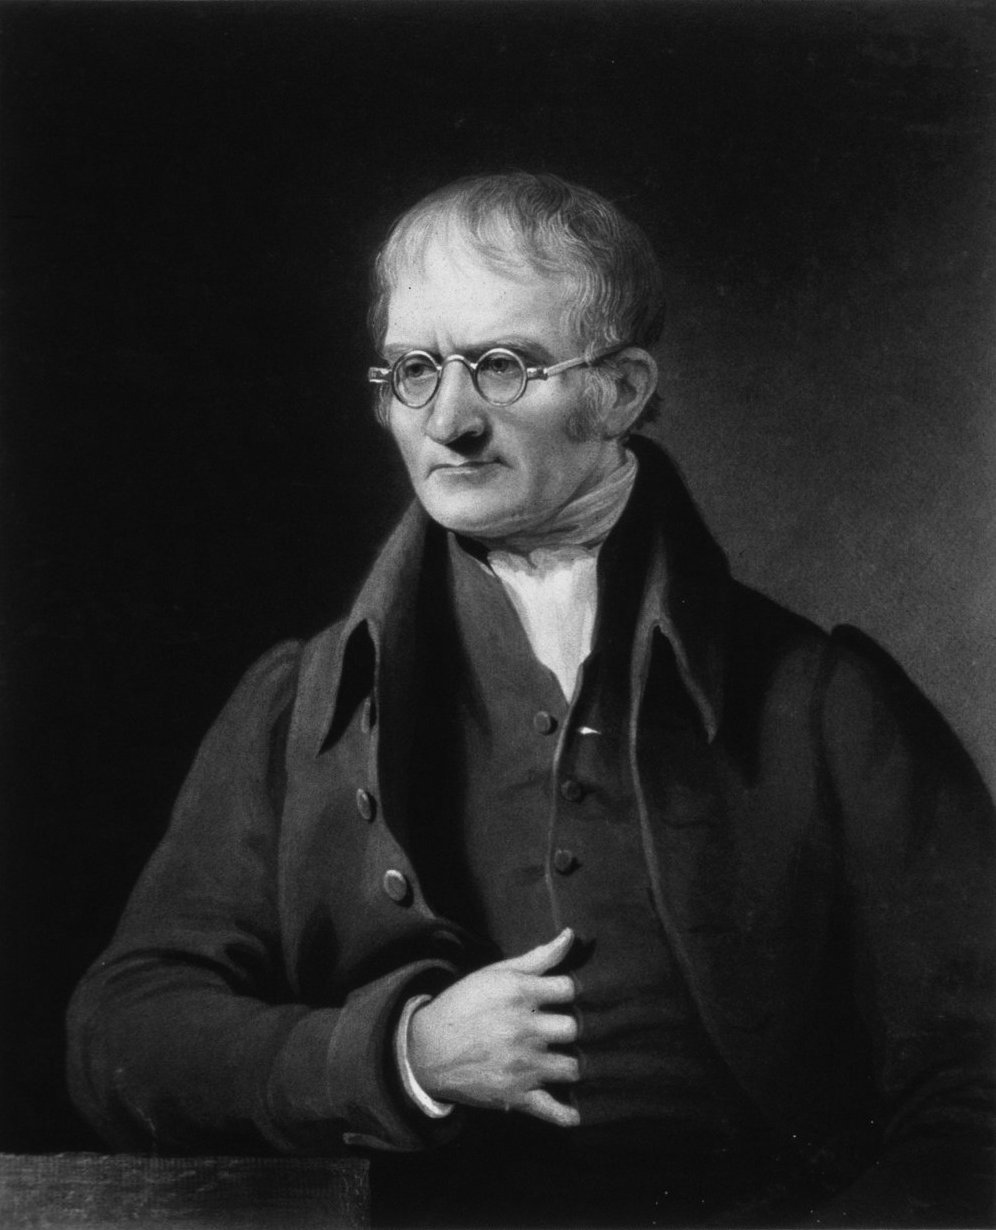
\includegraphics[width=\linewidth]{images/book1/dalton.jpg}

{\small John Dalton (1766--1844).}
\end{minipage}\hfill
\begin{minipage}[b]{0.66\linewidth}\centering
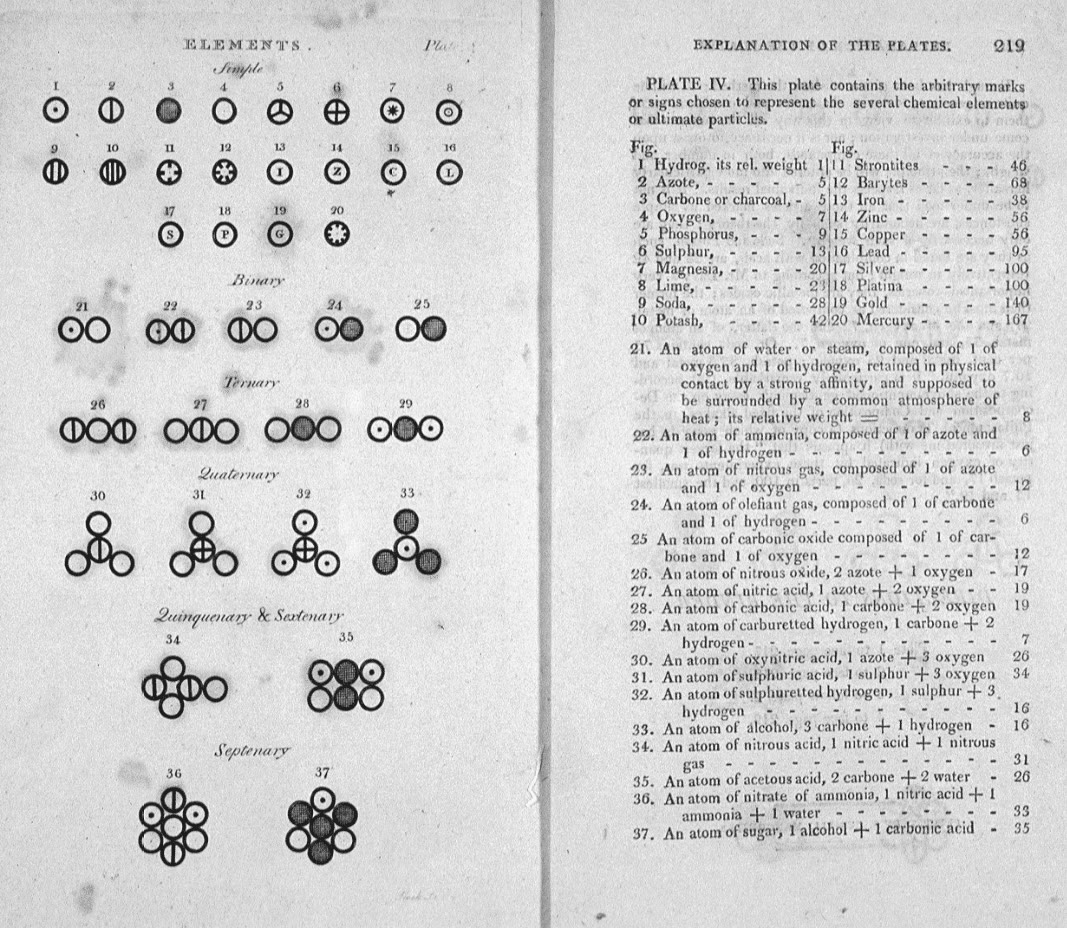
\includegraphics[width=\linewidth]{images/book1/dalton-symbols.jpg}

{\small A tabela de Dalton de 1808: a água dele, sinal 21, é um círculo
de hidrogênio ao lado de um de oxigênio.}
\end{minipage}
\end{omfigure}

\section{As moléculas}

\begin{definition}[Molécula]\label{def:g7:atoms-and-molecules:molecule}
Uma \emph{molécula}\index{molecula@molécula} é um grupo de \omterm{def:g7:atoms-and-molecules:atom}{átomos} firmemente
unidos. Uma molécula é o menor pedaço de uma substância que ainda é essa
substância: uma molécula de água é a menor quantidade possível de água.
\end{definition}

\begin{example}[Sete moléculas]\label{ex:g7:atoms-and-molecules:seven}
\begin{itemize}
  \item a \omterm{def:g7:atoms-and-molecules:molecule}{molécula} de \emph{hidrogênio}: dois \omterm{def:g7:atoms-and-molecules:atom}{átomos} de hidrogênio;
  \item a \omterm{def:g7:atoms-and-molecules:molecule}{molécula} de \emph{oxigênio}, que respiramos: dois \omterm{def:g7:atoms-and-molecules:atom}{átomos} de
        oxigênio;
  \item a \omterm{def:g7:atoms-and-molecules:molecule}{molécula} de \emph{nitrogênio}, quatro quintos do \omterm{def:g4:air-a-mixture-of-gases:air}{ar}: dois
        \omterm{def:g7:atoms-and-molecules:atom}{átomos} de nitrogênio;
  \item a \omterm{def:g7:atoms-and-molecules:molecule}{molécula} de \emph{água}: dois \omterm{def:g7:atoms-and-molecules:atom}{átomos} de hidrogênio e um \omterm{def:g7:atoms-and-molecules:atom}{átomo}
        de oxigênio;
  \item a \omterm{def:g7:atoms-and-molecules:molecule}{molécula} de \emph{dióxido de carbono}, que expiramos: um \omterm{def:g7:atoms-and-molecules:atom}{átomo}
        de carbono e dois \omterm{def:g7:atoms-and-molecules:atom}{átomos} de oxigênio;
  \item a \omterm{def:g7:atoms-and-molecules:molecule}{molécula} de \emph{metano}, a parte principal do gás natural
        queimado nos fogões a gás: um \omterm{def:g7:atoms-and-molecules:atom}{átomo} de carbono e quatro \omterm{def:g7:atoms-and-molecules:atom}{átomos} de
        hidrogênio;
  \item a \omterm{def:g7:atoms-and-molecules:molecule}{molécula} de \emph{óxido nitroso}, um gás anestésico: dois
        \omterm{def:g7:atoms-and-molecules:atom}{átomos} de nitrogênio e um \omterm{def:g7:atoms-and-molecules:atom}{átomo} de oxigênio.
\end{itemize}
\end{example}

\begin{omfigure}
\begin{tikzpicture}[font=\small]
  % hydrogen
  \begin{scope}[xshift=0cm]
    \node[aH] (a) at (-0.25,0) {}; \node[aH] (b) at (0.25,0) {};
    \begin{scope}[on background layer]\draw[bond] (a.center) -- (b.center);\end{scope}
    \node at (0,-1.05) {hidrogênio};
  \end{scope}
  % oxygen
  \begin{scope}[xshift=2.6cm]
    \node[aO] (a) at (-0.33,0) {}; \node[aO] (b) at (0.33,0) {};
    \begin{scope}[on background layer]
      \draw[bond, line width=1.1pt] ([yshift=1.6pt]a.center) -- ([yshift=1.6pt]b.center);
      \draw[bond, line width=1.1pt] ([yshift=-1.6pt]a.center) -- ([yshift=-1.6pt]b.center);
    \end{scope}
    \node at (0,-1.05) {oxigênio};
  \end{scope}
  % nitrogen
  \begin{scope}[xshift=5.2cm]
    \node[aN] (a) at (-0.33,0) {}; \node[aN] (b) at (0.33,0) {};
    \begin{scope}[on background layer]
      \foreach \d in {-2.4,0,2.4}
        \draw[bond, line width=0.9pt] ([yshift=\d pt]a.center) -- ([yshift=\d pt]b.center);
    \end{scope}
    \node at (0,-1.05) {nitrogênio};
  \end{scope}
  % water
  \begin{scope}[xshift=7.8cm, yshift=0.2cm]
    \node[aO] (o) at (0,0) {};
    \node[aH] (h1) at (-0.62,-0.48) {}; \node[aH] (h2) at (0.62,-0.48) {};
    \begin{scope}[on background layer]
      \draw[bond] (o.center) -- (h1.center); \draw[bond] (o.center) -- (h2.center);
    \end{scope}
    \node at (0,-1.25) {água};
  \end{scope}
  % carbon dioxide
  \begin{scope}[xshift=0.9cm, yshift=-2.7cm]
    \node[aO] (a) at (-0.85,0) {}; \node[aC] (c) at (0,0) {}; \node[aO] (b) at (0.85,0) {};
    \begin{scope}[on background layer]
      \foreach \d in {-1.6,1.6} {
        \draw[bond, line width=1.1pt] ([yshift=\d pt]a.center) -- ([yshift=\d pt]c.center);
        \draw[bond, line width=1.1pt] ([yshift=\d pt]c.center) -- ([yshift=\d pt]b.center);}
    \end{scope}
    \node at (0,-1.05) {dióxido de carbono};
  \end{scope}
  % methane
  \begin{scope}[xshift=4.4cm, yshift=-2.6cm]
    \node[aC] (c) at (0,0) {};
    \node[aH] (h1) at (0,0.78) {};
    \node[aH] (h2) at (-0.74,-0.3) {};
    \node[aH] (h3) at (0.74,-0.3) {};
    \begin{scope}[on background layer]
      \draw[bond] (c.center) -- (h1.center); \draw[bond] (c.center) -- (h2.center);
      \draw[bond] (c.center) -- (h3.center);
    \end{scope}
    \draw[bond] (c.center) -- (0.22,-0.52);
    \node[aH] at (0.24,-0.58) {};
    \node at (0,-1.15) {metano};
  \end{scope}
  % nitrous oxide
  \begin{scope}[xshift=7.8cm, yshift=-2.7cm]
    \node[aN] (a) at (-0.8,0) {}; \node[aN] (b) at (0,0) {}; \node[aO] (c) at (0.8,0) {};
    \begin{scope}[on background layer]
      \foreach \d in {-1.6,1.6} {
        \draw[bond, line width=1.1pt] ([yshift=\d pt]a.center) -- ([yshift=\d pt]b.center);
        \draw[bond, line width=1.1pt] ([yshift=\d pt]b.center) -- ([yshift=\d pt]c.center);}
    \end{scope}
    \node at (0,-1.05) {óxido nitroso};
  \end{scope}
\end{tikzpicture}

{\small Modelos de bolas e varetas das sete \omterm{def:g7:atoms-and-molecules:molecule}{moléculas} do
\cref{ex:g7:atoms-and-molecules:seven}. Cada vareta representa uma
ligação entre dois \omterm{def:g7:atoms-and-molecules:atom}{átomos}; por que alguns \omterm{def:g7:atoms-and-molecules:atom}{átomos} compartilham duas ou
três varetas é explicado num capítulo mais adiante.}
\end{omfigure}

\begin{proposition}[Moléculas de uma substância pura e de uma mistura]\label{prop:g7:atoms-and-molecules:pure}
Numa \omterm{def:g6:pure-substances-and-mixtures:pure-substance}{substância pura} formada por \omterm{def:g7:atoms-and-molecules:molecule}{moléculas}, todas as \omterm{def:g7:atoms-and-molecules:molecule}{moléculas} são
idênticas: a água pura só contém \omterm{def:g7:atoms-and-molecules:molecule}{moléculas} de água. Uma \omterm{def:g6:pure-substances-and-mixtures:mixture}{mistura} contém
\omterm{def:g7:atoms-and-molecules:molecule}{moléculas} de vários tipos: o \omterm{def:g4:air-a-mixture-of-gases:air}{ar} é formado principalmente por \omterm{def:g7:atoms-and-molecules:molecule}{moléculas}
de nitrogênio e \omterm{def:g7:atoms-and-molecules:molecule}{moléculas} de oxigênio, cerca de quatro de nitrogênio
para cada uma de oxigênio, com alguns \omterm{def:g7:atoms-and-molecules:atom}{átomos} de argônio que ficam
isolados e pouquíssimas \omterm{def:g7:atoms-and-molecules:molecule}{moléculas} de dióxido de carbono.
\end{proposition}

\begin{omfigure}
\begin{tikzpicture}[font=\small,
    sN/.style={aN, minimum size=3.0mm}, sO/.style={aO, minimum size=2.9mm},
    sH/.style={aH, minimum size=2.1mm}, sAr/.style={om atom, ball color=cyan!60, minimum size=3.4mm}]
  % air
  \draw[omGlass, line width=0.6pt] (0,0) rectangle (3.4,3.4);
  \foreach \x/\y/\r in {0.5/0.6/20, 1.6/0.4/-30, 2.8/0.7/75, 0.6/1.7/110,
                        2.0/1.5/10, 2.9/2.0/-60, 0.9/2.8/40, 2.1/2.9/-15}
    \node[sN] at ($(\x,\y)+(\r:0.12)$) {} node[sN] at ($(\x,\y)+(\r+180:0.12)$) {};
  \foreach \x/\y/\r in {1.3/1.1/60, 1.6/2.3/-40}
    \node[sO] at ($(\x,\y)+(\r:0.12)$) {} node[sO] at ($(\x,\y)+(\r+180:0.12)$) {};
  \node[sAr] at (2.9,3.0) {};
  \node[anchor=north] at (1.7,-0.1) {\textbf{ar}: uma mistura};
  % water
  \begin{scope}[xshift=5.2cm]
    \draw[omGlass, line width=0.6pt] (0,0) rectangle (3.4,3.4);
    \foreach \x in {0,1,2,3,4} \foreach \y in {0,1,2,3,4} {
      \pgfmathsetmacro{\ang}{mod(73*\x+41*\y,360)}
      \begin{scope}[shift={({0.36+0.67*\x},{0.4+0.66*\y})}, rotate=\ang]
        \node[sH] at (-0.16,-0.12) {}; \node[sH] at (0.16,-0.12) {};
        \node[sO] at (0,0) {};
      \end{scope}}
    \node[anchor=north] at (1.7,-0.1) {\textbf{água}: uma substância pura};
  \end{scope}
\end{tikzpicture}

{\small Um zoom enorme. À esquerda: no \omterm{def:g4:air-a-mixture-of-gases:air}{ar}, as \omterm{def:g7:atoms-and-molecules:molecule}{moléculas} de nitrogênio
(azuis) são muito mais numerosas que as de oxigênio (vermelhas), e um
\omterm{def:g7:atoms-and-molecules:atom}{átomo} de argônio (azul-claro) viaja sozinho; as \omterm{def:g7:atoms-and-molecules:molecule}{moléculas} de um gás
ficam afastadas umas das outras. À direita: na água líquida, as
\omterm{def:g7:atoms-and-molecules:molecule}{moléculas} são todas idênticas e se tocam.}
\end{omfigure}

\section{As fórmulas químicas}

\begin{definition}[Fórmula química]\label{def:g7:atoms-and-molecules:formula}
A \emph{fórmula química}\index{formula quimica@fórmula química} de uma \omterm{def:g7:atoms-and-molecules:molecule}{molécula} lista os
\omterm{def:g7:atoms-and-molecules:symbol}{símbolos} dos seus \omterm{def:g7:atoms-and-molecules:atom}{átomos}, cada um seguido de um pequeno número escrito
abaixo da linha --- o \emph{índice}\index{indice@índice} --- que diz quantos
\omterm{def:g7:atoms-and-molecules:atom}{átomos} desse tipo a \omterm{def:g7:atoms-and-molecules:molecule}{molécula} contém. O índice 1 não é escrito.
\end{definition}

\begin{example}[As sete fórmulas]\label{ex:g7:atoms-and-molecules:formulas}
As \omterm{def:g7:atoms-and-molecules:molecule}{moléculas} do \cref{ex:g7:atoms-and-molecules:seven} têm estas
fórmulas:
\begin{center}
\begin{tabular}{lcl}
\hline
\omterm{def:g7:atoms-and-molecules:molecule}{molécula} & fórmula & \omterm{def:g7:atoms-and-molecules:atom}{átomos} \\
\hline
hidrogênio & \ce{H2} & 2 de hidrogênio \\
oxigênio & \ce{O2} & 2 de oxigênio \\
nitrogênio & \ce{N2} & 2 de nitrogênio \\
água & \ce{H2O} & 2 de hidrogênio, 1 de oxigênio \\
dióxido de carbono & \ce{CO2} & 1 de carbono, 2 de oxigênio \\
metano & \ce{CH4} & 1 de carbono, 4 de hidrogênio \\
óxido nitroso & \ce{N2O} & 2 de nitrogênio, 1 de oxigênio \\
\hline
\end{tabular}
\end{center}
\end{example}

\begin{method}[Ler uma fórmula]\label{met:g7:atoms-and-molecules:read}
Para ler a fórmula de uma \omterm{def:g7:atoms-and-molecules:molecule}{molécula}:
\begin{enumerate}
  \item divida-a em \omterm{def:g7:atoms-and-molecules:symbol}{símbolos}: cada um começa com uma letra maiúscula;
  \item depois de cada \omterm{def:g7:atoms-and-molecules:symbol}{símbolo}, leia o \omterm{def:g7:atoms-and-molecules:formula}{índice} (sem \omterm{def:g7:atoms-and-molecules:formula}{índice} quer dizer 1);
  \item some os \omterm{def:g7:atoms-and-molecules:formula}{índices} para obter o número total de \omterm{def:g7:atoms-and-molecules:atom}{átomos}.
\end{enumerate}
Para \ce{C2H6O} (o etanol, o álcool das bebidas): 2 de carbono, 6 de
hidrogênio, 1 de oxigênio, 9 \omterm{def:g7:atoms-and-molecules:atom}{átomos} ao todo.
\end{method}

\begin{remark}[Um número na frente]\label{rem:g7:atoms-and-molecules:coefficient}
Um número escrito na frente de uma fórmula conta \omterm{def:g7:atoms-and-molecules:molecule}{moléculas}: \ce{3H2O}
quer dizer três \omterm{def:g7:atoms-and-molecules:molecule}{moléculas} de água, que juntas contêm 6 \omterm{def:g7:atoms-and-molecules:atom}{átomos} de
hidrogênio e 3 \omterm{def:g7:atoms-and-molecules:atom}{átomos} de oxigênio. Não confunda \ce{O2}, uma \omterm{def:g7:atoms-and-molecules:molecule}{molécula}
formada por dois \omterm{def:g7:atoms-and-molecules:atom}{átomos} de oxigênio, com \ce{2O}, dois \omterm{def:g7:atoms-and-molecules:atom}{átomos} de
oxigênio que não estão ligados.
\end{remark}

\begin{example}[O metano na cozinha]\label{ex:g7:atoms-and-molecules:methane}
O gás natural de um fogão a gás é principalmente metano, \ce{CH4}. Cada
uma das suas \omterm{def:g7:atoms-and-molecules:molecule}{moléculas} é um \omterm{def:g7:atoms-and-molecules:atom}{átomo} de carbono com quatro \omterm{def:g7:atoms-and-molecules:atom}{átomos} de
hidrogênio em volta. O gás é invisível e não tem cheiro: o cheiro de
``gás'' vem de uma substância acrescentada de propósito, para que um
vazamento seja percebido.
\end{example}

\begin{omfigure}
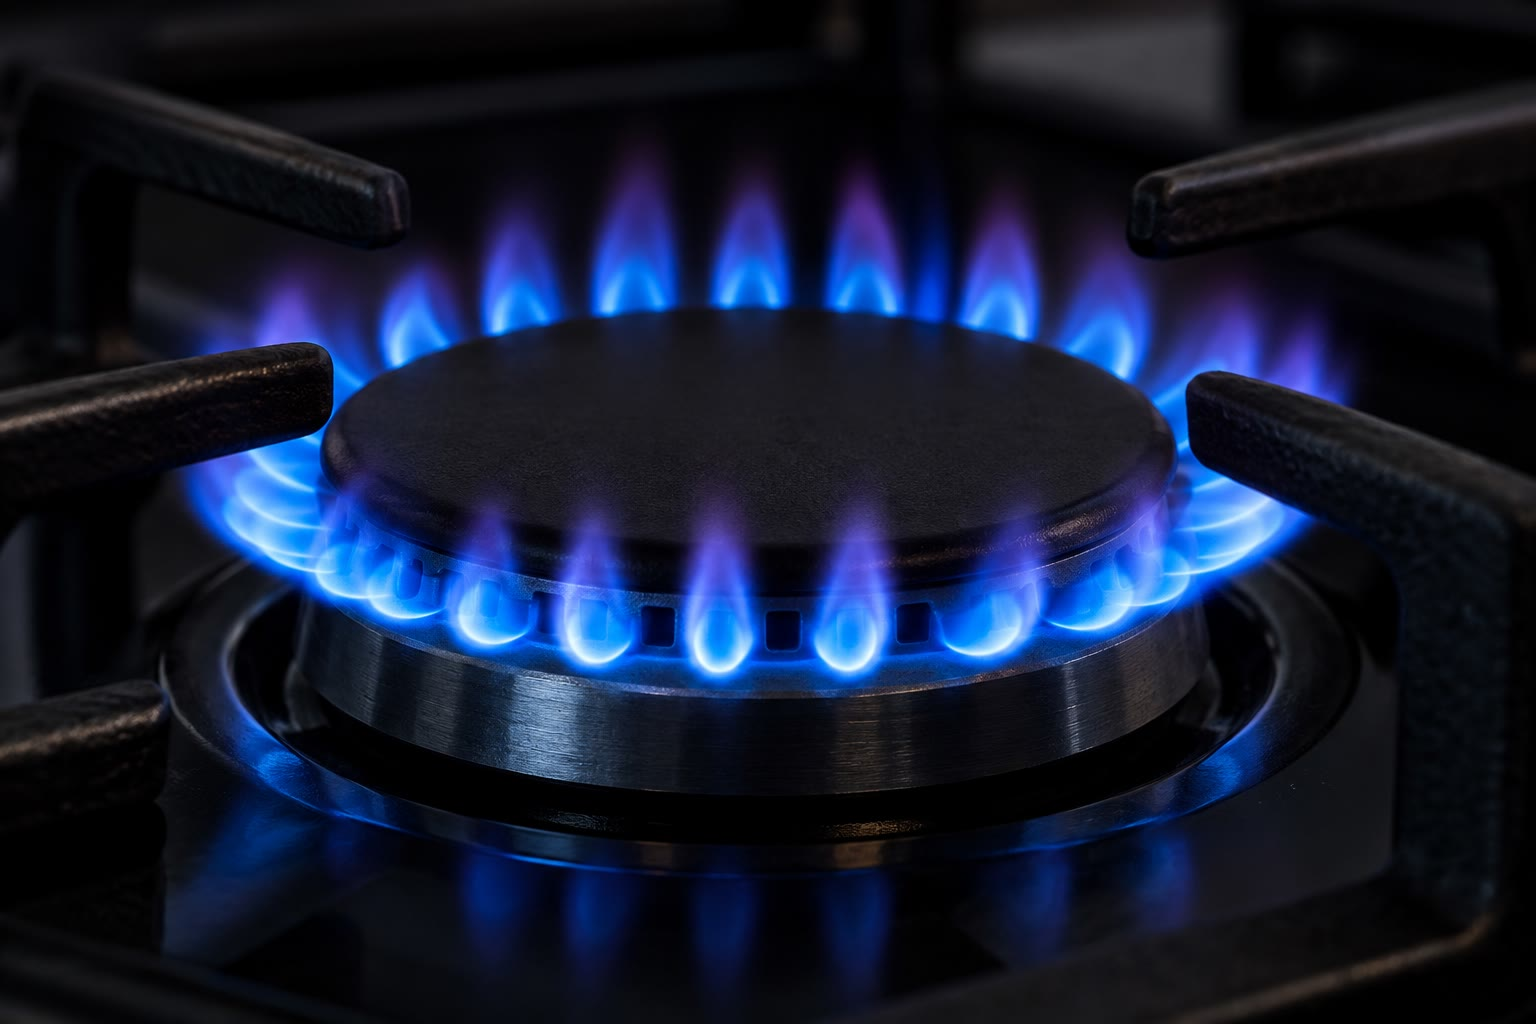
\includegraphics[width=0.5\linewidth]{images/book1/ai/g7-gas-flame.jpg}

{\small A chama azul de um fogão a gás: o metano do gás natural está
queimando.}
\end{omfigure}

\section{Os modelos moleculares}

\begin{remark}[Os modelos e as suas cores]\label{rem:g7:atoms-and-molecules:models}
Os químicos montam \emph{modelos moleculares} com bolas para os \omterm{def:g7:atoms-and-molecules:atom}{átomos} e
varetas para as ligações entre eles. As cores são uma convenção usada no
mundo inteiro --- carbono preto, hidrogênio branco, oxigênio vermelho,
nitrogênio azul --- e não a cor real dos \omterm{def:g7:atoms-and-molecules:atom}{átomos}: um \omterm{def:g7:atoms-and-molecules:atom}{átomo} isolado não
tem cor nenhuma. Um modelo também mostra a forma de uma \omterm{def:g7:atoms-and-molecules:molecule}{molécula}, o que
uma fórmula não faz: a \omterm{def:g7:atoms-and-molecules:molecule}{molécula} de água é angular, a \omterm{def:g7:atoms-and-molecules:molecule}{molécula} de
dióxido de carbono é linear.
\end{remark}

\begin{omfigure}
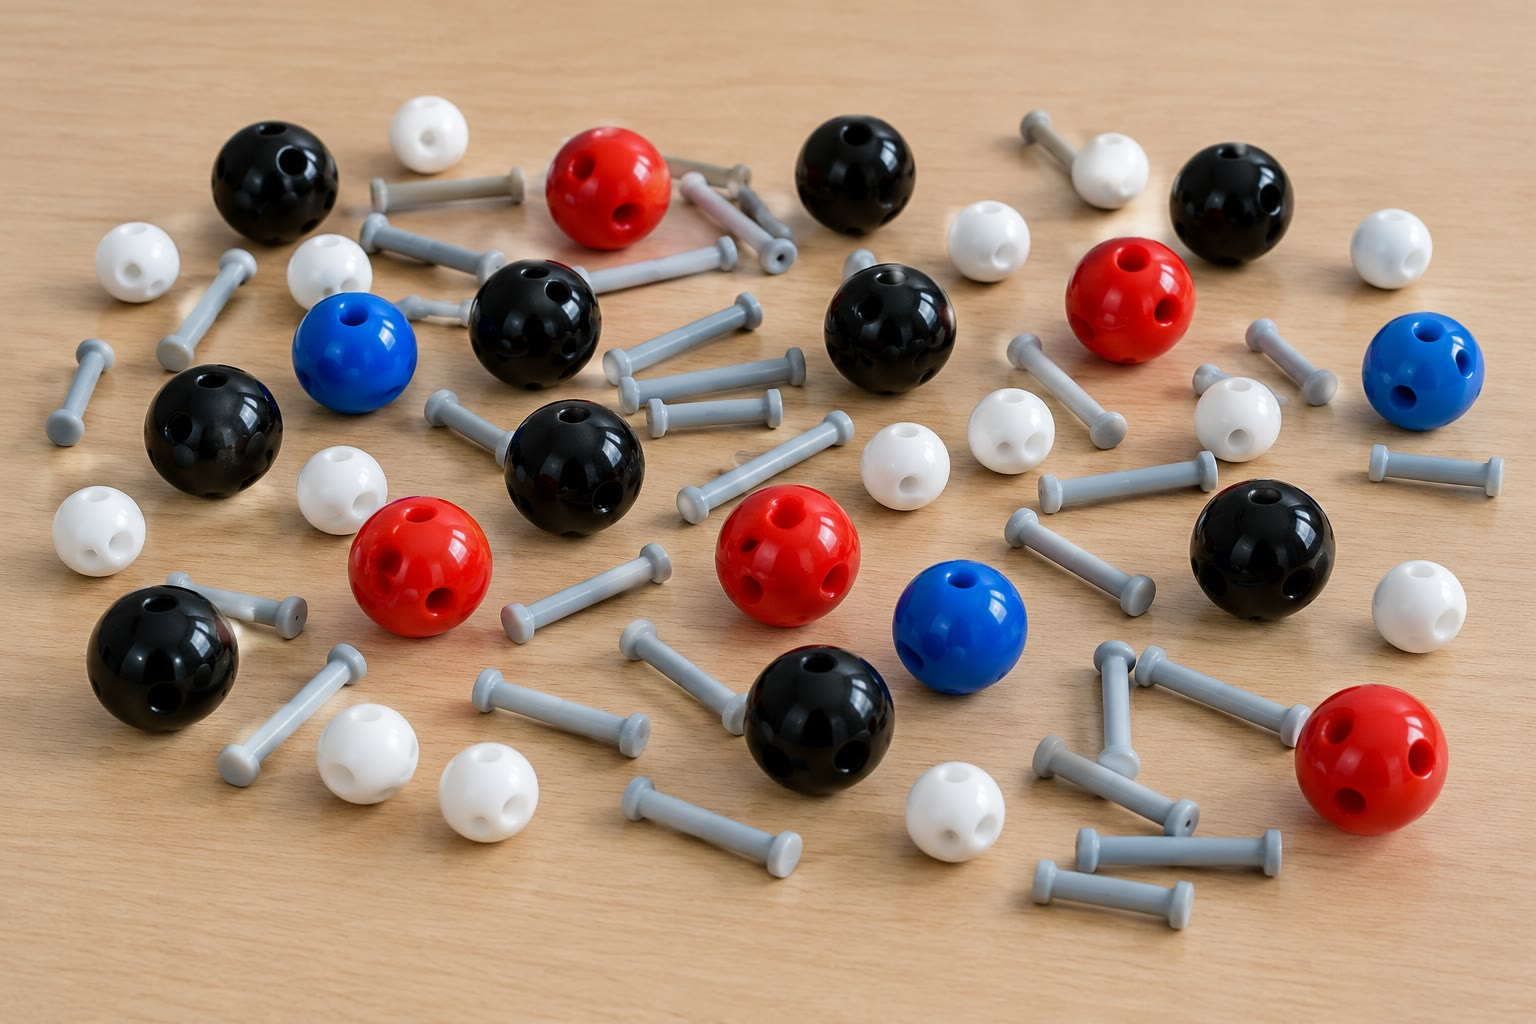
\includegraphics[width=0.5\linewidth]{images/book1/ai/g7-model-kit.jpg}

{\small Um kit de modelos moleculares: bolas para os \omterm{def:g7:atoms-and-molecules:atom}{átomos}, com furos
para as varetas que representam as ligações.}
\end{omfigure}

\begin{method}[Do modelo à fórmula]\label{met:g7:atoms-and-molecules:model}
Para escrever a fórmula de uma \omterm{def:g7:atoms-and-molecules:molecule}{molécula} a partir do seu modelo:
\begin{enumerate}
  \item dê o nome dos \omterm{def:g7:atoms-and-molecules:atom}{átomos} pelas cores deles;
  \item conte as bolas de cada cor;
  \item escreva os \omterm{def:g7:atoms-and-molecules:symbol}{símbolos} com as contagens como \omterm{def:g7:atoms-and-molecules:formula}{índices}, primeiro o
        carbono, depois o hidrogênio, depois os outros \omterm{def:g7:atoms-and-molecules:atom}{átomos} em ordem
        alfabética dos \omterm{def:g7:atoms-and-molecules:symbol}{símbolos}.
\end{enumerate}
Uma bola preta ligada a quatro brancas: um carbono, quatro hidrogênios,
\ce{CH4}.
\end{method}

\section{Exercícios}

\begin{exercise}[$\star$]\label{exo:g7:atoms-and-molecules:1}
O que é um \omterm{def:g7:atoms-and-molecules:atom}{átomo}? O que é uma \omterm{def:g7:atoms-and-molecules:molecule}{molécula}?
\end{exercise}

\begin{exercise}[$\star$]\label{exo:g7:atoms-and-molecules:2}
Dê os \omterm{def:g7:atoms-and-molecules:symbol}{símbolos} do hidrogênio, do carbono, do nitrogênio, do oxigênio, do
sódio e do ferro.
\end{exercise}

\begin{exercise}[$\star$]\label{exo:g7:atoms-and-molecules:3}
Quantos \omterm{def:g7:atoms-and-molecules:atom}{átomos} de cada tipo há numa \omterm{def:g7:atoms-and-molecules:molecule}{molécula} de dióxido de carbono,
\ce{CO2}? Quantos \omterm{def:g7:atoms-and-molecules:atom}{átomos} ao todo?
\end{exercise}

\begin{exercise}[$\star$]\label{exo:g7:atoms-and-molecules:4}
Dê o nome das \omterm{def:g7:atoms-and-molecules:molecule}{moléculas} \ce{H2O}, \ce{O2}, \ce{CH4} e \ce{N2}.
\end{exercise}

\begin{exercise}[$\star$]\label{exo:g7:atoms-and-molecules:5}
Uma \omterm{def:g7:atoms-and-molecules:molecule}{molécula} de dióxido de nitrogênio, um gás castanho presente no \omterm{def:g4:air-a-mixture-of-gases:air}{ar}
poluído, é formada por um \omterm{def:g7:atoms-and-molecules:atom}{átomo} de nitrogênio e dois \omterm{def:g7:atoms-and-molecules:atom}{átomos} de oxigênio.
Escreva a fórmula dela.
\end{exercise}

\begin{exercise}[$\star\star$]\label{exo:g7:atoms-and-molecules:6}
Explique a diferença entre \ce{O2} e \ce{2O}, e entre \ce{CO} e
\ce{Co}.
\end{exercise}

\begin{exercise}[$\star\star$]\label{exo:g7:atoms-and-molecules:7}
Quantos \omterm{def:g7:atoms-and-molecules:atom}{átomos} de hidrogênio e quantos \omterm{def:g7:atoms-and-molecules:atom}{átomos} de oxigênio há em
\ce{3H2O}? E em \ce{5O2}?
\end{exercise}

\begin{exercise}[$\star\star$]\label{exo:g7:atoms-and-molecules:8}
Um modelo é formado por uma bola preta ligada a duas bolas vermelhas. Dê
o nome dos \omterm{def:g7:atoms-and-molecules:atom}{átomos}, escreva a fórmula e dê o nome da \omterm{def:g7:atoms-and-molecules:molecule}{molécula}.
\end{exercise}

\begin{exercise}[$\star\star$]\label{exo:g7:atoms-and-molecules:9}
Na tabela de Dalton, a água é formada por um \omterm{def:g7:atoms-and-molecules:atom}{átomo} de hidrogênio e um
\omterm{def:g7:atoms-and-molecules:atom}{átomo} de oxigênio. Escreva a fórmula que Dalton tinha em mente, e diga
quantos \omterm{def:g7:atoms-and-molecules:atom}{átomos} faltam na \omterm{def:g7:atoms-and-molecules:molecule}{molécula} de água dele.
\end{exercise}

\begin{exercise}[$\star\star$]\label{exo:g7:atoms-and-molecules:10}
A água pura é uma \omterm{def:g6:pure-substances-and-mixtures:mixture}{mistura}? E o \omterm{def:g4:air-a-mixture-of-gases:air}{ar}? Responda descrevendo as \omterm{def:g7:atoms-and-molecules:molecule}{moléculas} que
cada um contém.
\end{exercise}

\begin{exercise}[$\star\star\star$]\label{exo:g7:atoms-and-molecules:11}
Um \omterm{def:g7:atoms-and-molecules:atom}{átomo} de hidrogênio mede cerca de um décimo de milionésimo de
milímetro de diâmetro. Quantos \omterm{def:g7:atoms-and-molecules:atom}{átomos} de hidrogênio, lado a lado,
formariam uma linha de \qty{1}{cm}? E uma linha do comprimento de um
campo de futebol, \qty{100}{m}?
\end{exercise}

\begin{exercise}[$\star\star\star$]\label{exo:g7:atoms-and-molecules:12}
A glicose, o açúcar que alimenta as nossas células, tem a fórmula
\ce{C6H12O6}. Quantos \omterm{def:g7:atoms-and-molecules:atom}{átomos} uma \omterm{def:g7:atoms-and-molecules:molecule}{molécula} de glicose contém? Que
porcentagem deles são \omterm{def:g7:atoms-and-molecules:atom}{átomos} de hidrogênio? Que porcentagem são \omterm{def:g7:atoms-and-molecules:atom}{átomos}
de carbono?
\end{exercise}

\section{Problema: os átomos de uma respiração}

\begin{problem}[{Problema de fim de semana --- contar os átomos de uma
porção de ar respirado, antes e depois de passar pelos nossos pulmões}]
\label{pb:g7:atoms-and-molecules:1}
% ledger: air:N2, air:O2, air:Ar (78.08 / 20.95 / 0.93 rounded to 78 / 21 / 1),
% breath:O2, breath:CO2, breath:N2 (expired air: 16 / 4 / 78, water vapour removed)
O nitrogênio passa pelos pulmões sem mudar, por isso ele é uma boa
referência. No \omterm{def:g4:air-a-mixture-of-gases:air}{ar} seco, para cada 78 \omterm{def:g7:atoms-and-molecules:molecule}{moléculas} de nitrogênio há cerca de
21 \omterm{def:g7:atoms-and-molecules:molecule}{moléculas} de oxigênio e 1 \omterm{def:g7:atoms-and-molecules:atom}{átomo} de argônio: 100 partículas (\omterm{def:g7:atoms-and-molecules:molecule}{moléculas}
ou \omterm{def:g7:atoms-and-molecules:atom}{átomos} isolados) ao todo. No \omterm{def:g4:air-a-mixture-of-gases:air}{ar} expirado, depois de retirado o vapor
de água, as mesmas 78 \omterm{def:g7:atoms-and-molecules:molecule}{moléculas} de nitrogênio vêm acompanhadas de cerca
de 16 \omterm{def:g7:atoms-and-molecules:molecule}{moléculas} de oxigênio, 4 \omterm{def:g7:atoms-and-molecules:molecule}{moléculas} de dióxido de carbono e 1 \omterm{def:g7:atoms-and-molecules:atom}{átomo}
de argônio.

\medskip
\noindent\textbf{Parte I --- O \omterm{def:g4:air-a-mixture-of-gases:air}{ar} que inspiramos.}
\begin{enumerate}
  \item Escreva as fórmulas das \omterm{def:g7:atoms-and-molecules:molecule}{moléculas} de nitrogênio, de oxigênio e de
        dióxido de carbono, e dê o número de \omterm{def:g7:atoms-and-molecules:atom}{átomos} de cada uma.
  \item O argônio é contado em \omterm{def:g7:atoms-and-molecules:atom}{átomos}, não em \omterm{def:g7:atoms-and-molecules:molecule}{moléculas}. O que isso nos
        diz sobre o argônio?
  \item Nessas 100 partículas de \omterm{def:g4:air-a-mixture-of-gases:air}{ar} inspirado, quantos \omterm{def:g7:atoms-and-molecules:atom}{átomos} de
        nitrogênio há? Quantos \omterm{def:g7:atoms-and-molecules:atom}{átomos} de oxigênio?
  \item Quantos \omterm{def:g7:atoms-and-molecules:atom}{átomos} há ao todo nessas 100 partículas?
  \item Que porcentagem desses \omterm{def:g7:atoms-and-molecules:atom}{átomos} são \omterm{def:g7:atoms-and-molecules:atom}{átomos} de nitrogênio? Arredonde
        para o número inteiro mais próximo.
\end{enumerate}

\medskip
\noindent\textbf{Parte II --- O \omterm{def:g4:air-a-mixture-of-gases:air}{ar} que expiramos.}
\begin{enumerate}[resume]
  \item No \omterm{def:g4:air-a-mixture-of-gases:air}{ar} expirado que acompanha as mesmas 78 \omterm{def:g7:atoms-and-molecules:molecule}{moléculas} de
        nitrogênio, quantos \omterm{def:g7:atoms-and-molecules:atom}{átomos} de oxigênio há dentro das \omterm{def:g7:atoms-and-molecules:molecule}{moléculas} de
        oxigênio? Dentro das \omterm{def:g7:atoms-and-molecules:molecule}{moléculas} de dióxido de carbono? Ao todo?
  \item Compare com a questão 3. Quantos \omterm{def:g7:atoms-and-molecules:atom}{átomos} de oxigênio faltam? Para
        dentro de que \omterm{def:g7:atoms-and-molecules:molecule}{molécula}, fabricada no corpo a partir do hidrogênio
        dos alimentos e retirada aqui junto com o vapor de água, eles
        foram?
  \item Quantos \omterm{def:g7:atoms-and-molecules:atom}{átomos} de carbono há no \omterm{def:g4:air-a-mixture-of-gases:air}{ar} inspirado? E no \omterm{def:g4:air-a-mixture-of-gases:air}{ar} expirado?
  \item O \omterm{def:g4:air-a-mixture-of-gases:air}{ar} não traz nenhum \omterm{def:g7:atoms-and-molecules:atom}{átomo} de carbono para os pulmões. De onde
        podem vir os \omterm{def:g7:atoms-and-molecules:atom}{átomos} de carbono do \omterm{def:g4:air-a-mixture-of-gases:air}{ar} expirado? (Pense no que o
        corpo usa para viver.)
  \item Quantas \omterm{def:g7:atoms-and-molecules:molecule}{moléculas} de oxigênio desapareceram, e quantas \omterm{def:g7:atoms-and-molecules:molecule}{moléculas}
        de dióxido de carbono apareceram?
\end{enumerate}

\medskip
\noindent\textbf{Parte III --- A contagem.}
\begin{enumerate}[resume]
  \item Descreva o modelo de bolas e varetas de cada um dos quatro tipos
        de partícula do \omterm{def:g4:air-a-mixture-of-gases:air}{ar} expirado, com as cores das bolas (o argônio é
        representado por uma única bola azul-clara).
  \item Quantos \omterm{def:g7:atoms-and-molecules:atom}{átomos} há ao todo no \omterm{def:g4:air-a-mixture-of-gases:air}{ar} expirado seco? Quantos \omterm{def:g7:atoms-and-molecules:atom}{átomos} ele
        tem a mais do que o \omterm{def:g4:air-a-mixture-of-gases:air}{ar} inspirado? Explique a diferença com os
        \omterm{def:g7:atoms-and-molecules:atom}{átomos} de carbono ganhos e os \omterm{def:g7:atoms-and-molecules:atom}{átomos} de oxigênio que faltam.
\end{enumerate}
\end{problem}
